\begin{frame}{Por que aprender comandos do terminal?}
  \begin{columns}
    \column{0.5\textwidth}
    \begin{itemize}
      \item Muitas ferramentas são otimizadas para uso via terminal, como Docker, SSH, FFmpeg e Git.
      \item Entender o terminal torna operações mais rápidas e repetíveis.
      \item Automatização de tarefas e scripts dependem do terminal.
    \end{itemize}
    \column{0.5\textwidth}
    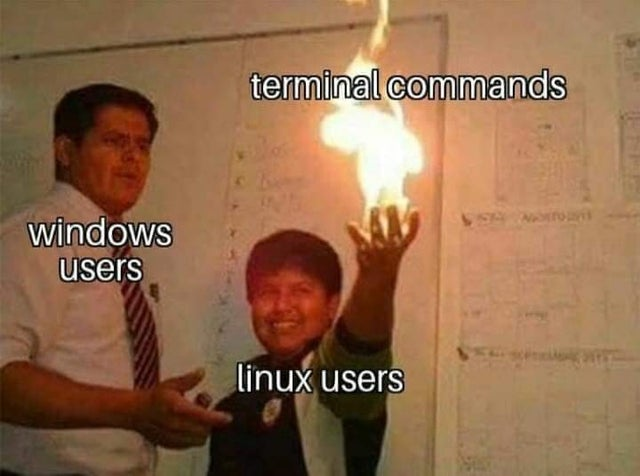
\includegraphics[width=\linewidth]{terminal.jpg}
  \end{columns}
\end{frame}

\begin{frame}{Comandos básicos do Linux}
  \begin{columns}
    \column{0.5\textwidth}
    \begin{block}{\texttt{pwd}: mostra o diretório atual}
      \texttt{pwd}
    \end{block}

    \begin{block}{\texttt{mkdir}: cria um diretório}
      \texttt{mkdir aula-linux}
    \end{block}

    \begin{block}{\texttt{ls}: lista arquivos e diretórios}
      \texttt{ls}
    \end{block}

    \begin{block}{\texttt{cd}: entra em um diretório}
      \texttt{cd aula-linux}
    \end{block}

    \begin{block}{\texttt{echo}: exibe um texto}
      \texttt{echo "Hello World"}
    \end{block}

    \column{0.5\textwidth}
    \centering
    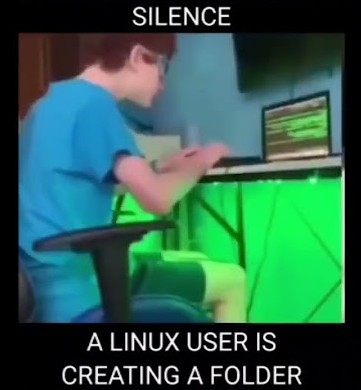
\includegraphics[width=0.9\linewidth]{linux-user.jpg}
  \end{columns}
\end{frame}

\begin{frame}
  \begin{columns}
    \column{0.5\textwidth}
    \begin{block}{\texttt{>} (Output Redirection): redireciona a saída para um arquivo}
      \texttt{echo "Hello World" \ > mensagem.txt}
    \end{block}

    \begin{block}{\texttt{ls}: lista arquivos e diretórios}
      \texttt{ls}
    \end{block}

    \begin{block}{\texttt{cat}: mostra o conteúdo de um arquivo}
      \texttt{cat mensagem.txt}
    \end{block}

    \begin{block}{\texttt{rm}: remove um arquivo}
      \texttt{rm mensagem.txt}
    \end{block}

    \begin{block}{\texttt{rmdir}: remove um diretório vazio}
      \texttt{rmdir aula-linux}
    \end{block}

    \column{0.5\textwidth}
    \centering
    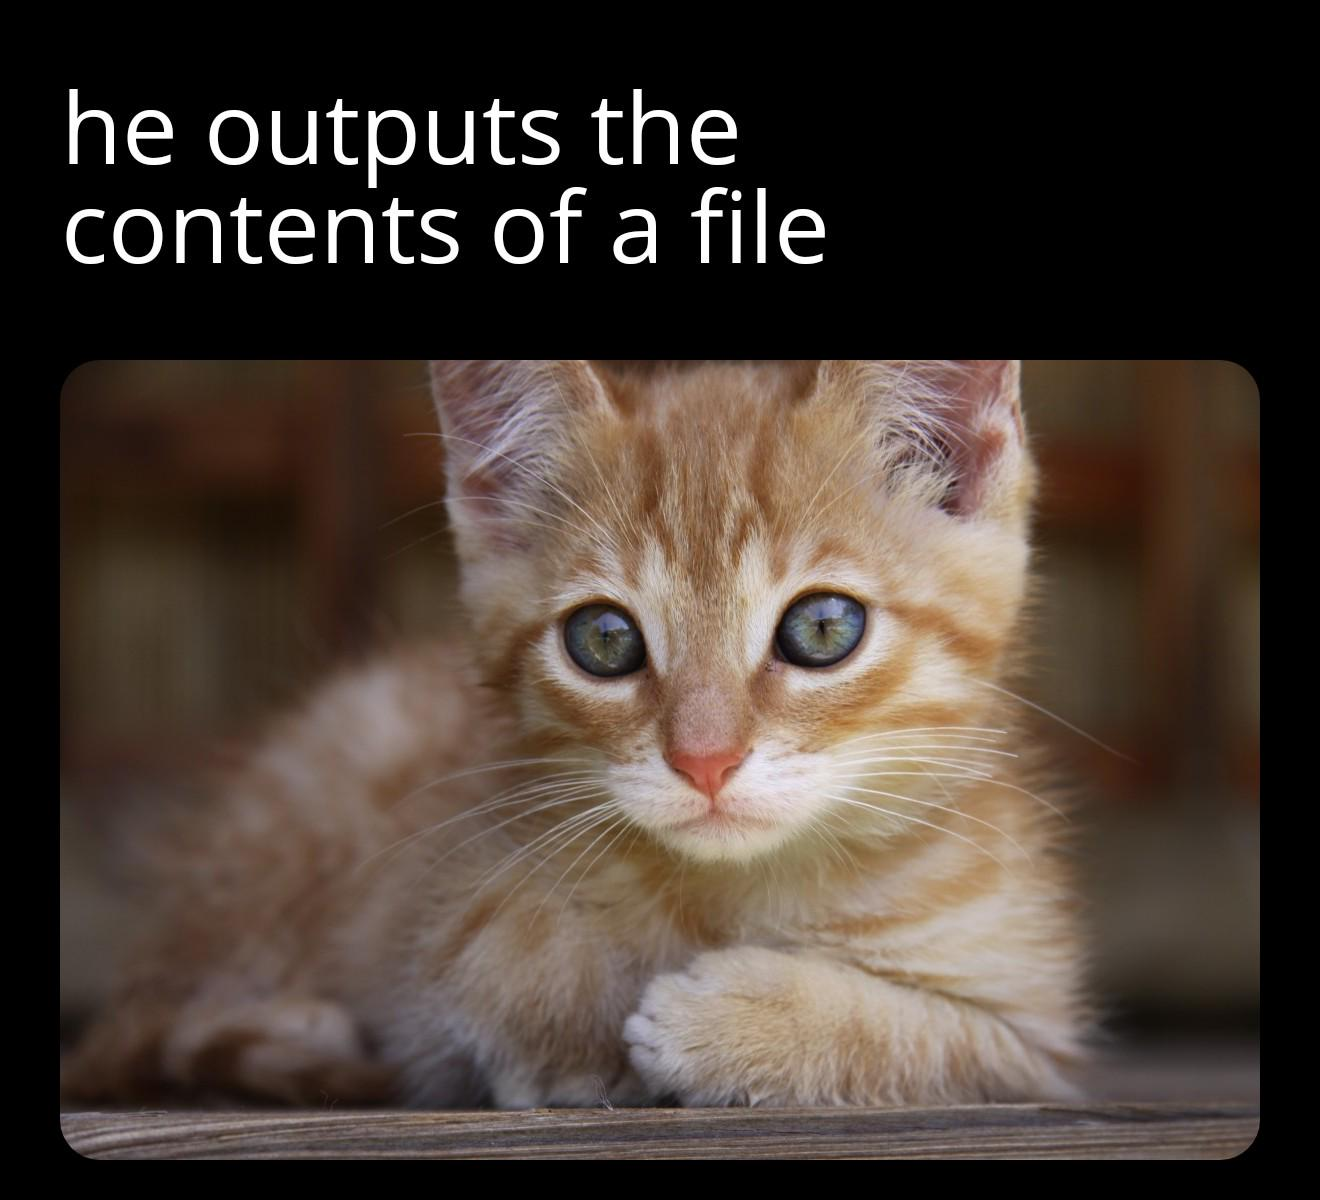
\includegraphics[width=\linewidth]{cat.jpeg}
  \end{columns}
\end{frame}

\begin{frame}
  \begin{block}{\texttt{diff}: compara dois arquivos}
    \texttt{diff arquivo1.txt arquivo2.txt}
  \end{block}
  \begin{block}{\texttt{patch}: aplica alterações em um arquivo}
    \texttt{diff -u arquivo1.txt arquivo2.txt > alteracoes.patch}

    \vspace{0.2cm}
    Cria um arquivo com as diferenças entre as duas versões.

    \vspace{0.3cm}
    \texttt{patch arquivo1.txt < alteracoes.patch}

    \vspace{0.2cm}
    Aplica as alterações de \texttt{alteracoes.patch} em \texttt{arquivo1.txt}.
  \end{block}

  \begin{block}{\texttt{sha256sum}: calcula o hash SHA-256}
    \texttt{sha256sum arquivo1.txt}

    \vspace{0.3cm}
    Gera uma sequência hexadecimal que identifica o conteúdo do arquivo (hash).
  \end{block}
\end{frame}
